%\vspace{12pt}
\section{Applications}
The application of this material is as a solid electrolyte, connecting cathode and anode of a cell and transporting ions. Solid electrolyte materials are used to either generate an electric potential from an applied chemical potential across the membrane, or vice versa. A concentration gradient for example can drive ionic species through the electrolyte while the associated electron current diverts through a resistive load until the reaction is complete. This is the essential function of a fuel cell or hydrogen sensor. Alternatively, an applied electric potential will create an electric field that will drive the ions through the membrane, even against a concentration gradient, functioning as for example a hydrogen pump. 

The solid electrolyte material serves three principal purposes in any application or device. First, the material itself acts as a gas separation barrier, maintaining separate compartments for the reaction gases. In the case of hydrogen fuel cells, the membrane separates the compartments for hydrogen (or hydrocarbon) and oxygen gas, as well as the water vapor exhaust. Second, the membrane blocks conduction of electrons, directing them instead to the connected electrical circuit for use. This is accomplished by way of a triple phase boundary at the anode and cathode that allows gases to interact with the solid phase but provides separate pathways for the flow of ions and electrons. Third, the membrane facilitates incorporation and conduction of specific ion species, balancing the load of electrons, and completion of the driving chemical reaction. An additional practical benefit of solid electrolytes is that they can serve as a structural feature of the cell, supporting anode or cathode materials and other conduction structures if made thick enough.

Fuel cells operate on the principle of the conversion of chemical energy directly to electrical energy, without the use of fuel combustion to power traditional electrical generators. Electrical energy is used to provide the useful work, while reaction products are exhausted through one of the gas chambers. Fuel cells require a separation of the reactants, in most cases hydrogen and oxygen by an electrolyte permeable to ions but not electrons. The efficiency of the operation depends upon the conductivity of the electrolyte, while the widespread adoption and use depend on stability of the materials and the operating temperatures that are required.
\begin{figure}
    \centering
    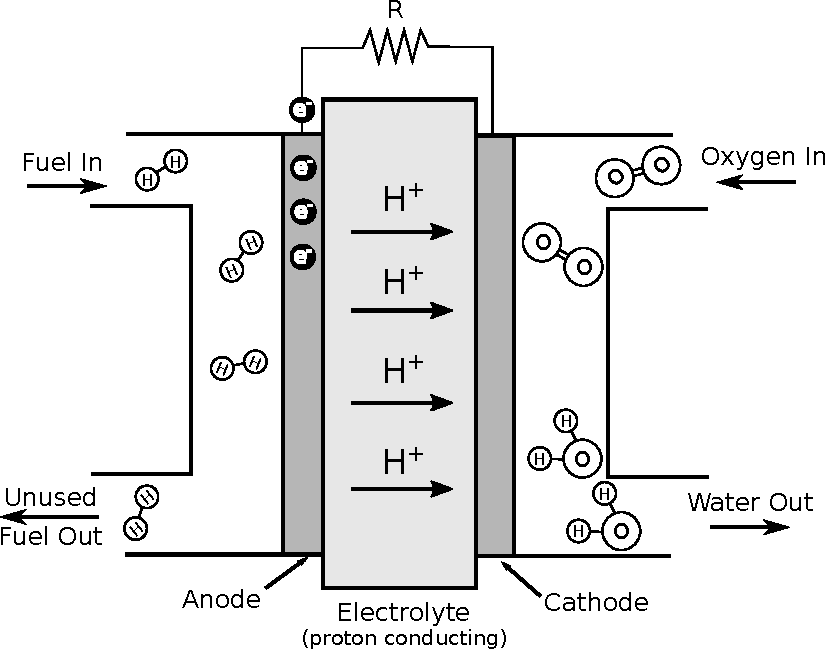
\includegraphics[width=.8\linewidth]{Figures/fuelCell2.pdf}
    \caption{Schematic of a protonic fuel cell.}
    \label{back:fig:fuelCell}
\end{figure}

Solid oxide electrolyte fuel cells operate by either the transport of oxide ions, or protons. Protonic fuel cells, as shown in Figure \ref{back:fig:fuelCell}, offer the opportunity for lower operating temperatures due to the lower activation energy of protonic conduction relative to oxide ion conduction. As an additional practical benefit of protonic cells, the water vapor that is ultimately formed as exhaust will occur on the oxygen side of the cell, and therefore the exhaust will not dilute the fuel side of the cell.

Currently, the oxide ion conductor yttria stabilized zirconia (YSZ) is the industry standard for electrolyte performance in the solid oxide fuel cell class. This class offers the longest lifetime and highest power outputs compared to other types such as alkaline fuel cell or proton exchange membrane fuel cell. Oxygen vacancies are formed by the yttria doping, and this provides the mechanism for conduction at elevated temperatures. Yet these devices remain a niche product as large stationary power supplies for back up or remote power generation. The temperatures required to operate these fuel cells range from 900\textdegree C to 1100\textdegree C \cite{Zhang2018}. These temperatures limit cycle lifetimes and require long startup times with expensive interconnects capable of withstanding thermal cycling. Figure \ref{back:fig:ArrheniusComparison} shows the conductivity values of YSZ along with several other materials under investigation for use as electrolytes in solid oxide fuel cells. 

\begin{figure}
    \centering
    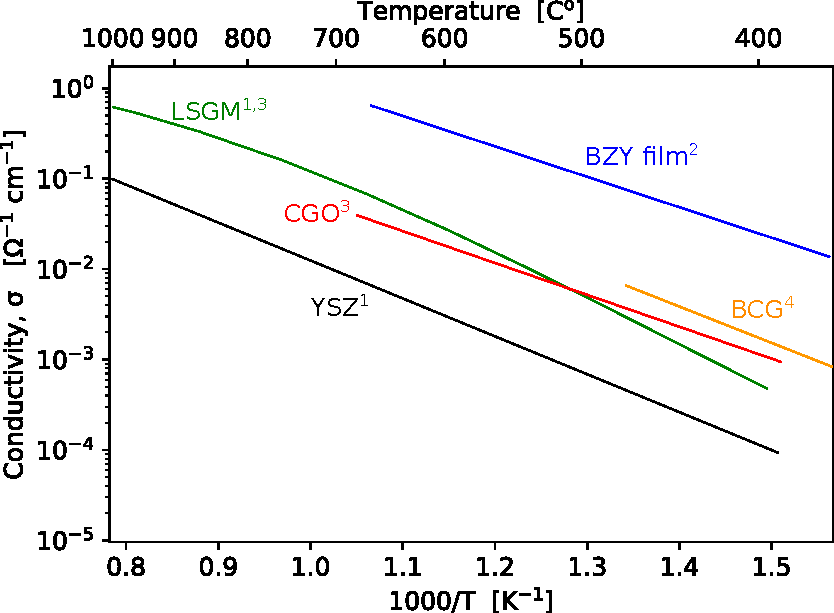
\includegraphics{Figures/ArrheniusComparison.pdf}
    \caption{A comparison of proton and oxide ion conducting materials. Acronyms: YSZ - yttria stabalized zirconia; CGO - ceria doped with gadolinium; BCG - barium cerate doped with gadolinium; LSGM - lanthanum gallate doped with strontium and magnesium; BZY - barium zirconated doped with yttrium. Data from references 1: \textcite{Wincewicz2005}, 2: \textcite{Pergolesi2010}, 3: \textcite{Esposito2008}, 4: \textcite{Ishihara2000}.}
    \label{back:fig:ArrheniusComparison}
\end{figure}

For this reason, reducing the operating temperatures of fuel cells remains an important goal in their adoption and widespread use, as well as extension into smaller scales which may provide clean, renewable energy at even the domestic level. This overarching goal has been approached principally in two different ways, both of which are examined in this work. First and most obviously is the search for new materials with higher conductivity at lower temperatures. As already discussed, proton conducting electrolytes offer promise in this area if suitable dopants and synthesis methods can be established to promote function and stability. This can be measured in the reduction of activation energy, leading to higher conductivity at lower temperatures. Second, decreasing the thickness of the electrolyte to the very minimum that would still accomplish the goal of electronic and ionic separation as well as gas impermeability would offer a straightforward decrease in ohmic losses through the electrolyte.  